\documentclass[12pt]{article}
\usepackage{amsmath,amsthm,amssymb,scrextend}
\usepackage[margin=1in]{geometry}
\usepackage{pgfplots}
\pgfplotsset{compat=1.18}
\setlength{\parindent}{0pt}
\begin{document}
\newcommand{\ds}{\displaystyle}

\textbf{(i)}

$$
\mathrm{Min}(x^2,2x)=
\begin{cases}
x^2, & \quad x^2\leq2x\\
2x, & \quad  x^2>2x
\end{cases}
$$
\begin{align*}
&x^2\leq2x\implies x(x-2)\leq0\implies0\leq x\leq2\\
&x^2>2x \;\implies\; x>2 \text{ or } x<0
\end{align*}
$$
\mathrm{Min}(x^2,2x)=
\begin{cases}
x^2, &\quad  0\leq x\leq2\\
2x, & \quad x<0\text{ or }x>2
\end{cases}
$$

\begin{center}
\begin{tikzpicture}
\begin{axis}[
    axis lines=middle,
    xmin=-2.8, xmax=5.2,
    ymin=-5.5, ymax=7,
    width=11cm,
    height=8cm,
    axis line style={->, thick},
    xlabel={$x$},
    ylabel={$y$},
    ylabel style={at={(axis cs:0.12,4.7)}, anchor=south west},
    xlabel style={at={(axis description cs:0.98,0.40)}, anchor=west},
    ylabel style={at={(axis cs:-0.28,6.7)}, anchor=south},
    xtick={2},
    ytick={4},
    xticklabels={$2$},
    yticklabels={$4$},
    tick style={draw=none},
    enlargelimits=false,
    clip=false,
    samples=100
]
\addplot[domain=-2.5:0, thick] {2*x};
\addplot[domain=0:2, thick] {x^2};
\addplot[domain=2:4.1, thick] {2*x};
\addplot[dashed] coordinates {(2,0) (2,4)};
\addplot[dashed] coordinates {(0,4) (2,4)};
\node at (axis cs:0,0) [below left] {$0$};
\node at (axis cs:0.85,2.45) {$y=x^2$};
\node at (axis cs:-1.95,-2.65) {$y=2x$};
\node at (axis cs:3.85,6.45) {$y=2x$};
\end{axis}
\end{tikzpicture}
\end{center}

\bigskip\hrule\bigskip

\textbf{(ii)}

$$2\mathrm{Min}(x^2,2x)=5x-3$$

$$ \text{If} \ \displaystyle 0\leq x\leq2 \implies 2x^2=5x-3$$
$$(2x-3)(x-1)=0 \implies x=\frac32,\; 1$$

$$ \text{If}\ x<0 \ \text{or}\ x>2 \implies 4x=5x-3 \implies x=3$$

Hence,\hfill $\boxed{x=1,\; \frac32,\; 3}$\hfill $\;$

\bigskip\hrule\bigskip

\textbf{(iii)}

$$
\mathrm{Min}(x^3,4x)=
\begin{cases}
x^3, & \quad x^3\leq4x\\
4x, &\quad x^3>4x
\end{cases}
$$
$$x^3\leq4x\implies x(x-2)(x+2)\leq0$$

$$x\leq-2\quad\text{or}\quad0\leq x\leq2$$

\begin{align*}
\mathrm{Min}(x^3,4x)
&=
\begin{cases}
x^3, & x\leq-2\text{ or }0\leq x\leq2\\
4x, & -2<x<0\text{ or }x>2
\end{cases}
\end{align*}

\begin{align*}
\mathrm{Min}(x^2,2x)
&=
\begin{cases}
x^2, & 0\leq x\leq2\\
2x, & x<0\text{ or }x>2
\end{cases}
\end{align*}

When $m=2$

\begin{align*}
\text{1. }&x\leq-2:\quad x^3+2x=2x \text{ (rejected)}\\
\text{2. }&-2<x<0:\quad 4x+2x=2x \text{ (rejected)}\\
\text{3. }&0\leq x\leq2:\quad x^3+x^2=2x\implies x(x+2)(x-1)=0\\
\text{4. }&x>2:\quad 4x+2x=2x\text{ (rejected)}
\end{align*}
$$\text{So for }m=2:\ \boxed{x=0,\; 1}$$

When $m=6$

\begin{align*}
\text{1. }&x\leq-2:\quad x^3+2x=6x \implies x(x-2)(x+2)=0\implies x=-2\\
\text{2. }&-2<x<0:\quad 4x+2x=6x \implies x\in\mathbb{R} \ (-2<x<0)\\
\text{3. }&0\leq x\leq2:\quad x^3+x^2=6x \implies x(x+3)(x-2)=0\implies x=0, 2\\
\text{4. }&x>2:\quad 4x+2x=6x \implies x\in \mathbb{R}
\end{align*}

$$\text{So for }m=6:\ \boxed{-2\leq x\leq0\ \text{or}\  x\geq2}$$

\bigskip\hrule\bigskip

\textbf{(iv)}

$$y=2\mathrm{Min}(x^2,x^3)-5x$$

$$
y=
\begin{cases}
2x^2-5x, & \text{when }x\geq1\\
2x^3-5x, & \text{when }x<1
\end{cases}
$$

For $x\geq1$
$$\frac{dy}{dx}=4x-5=0\implies x=\frac54 $$
$$y=2x^2-5x=2\cdot\frac{25}{16}-5\cdot\frac54=-\frac{25}{8}$$

$$\frac{d^2y}{dx^2}=4>0\implies \left(\frac54,-\frac{25}{8}\right)\text{ is minimum point}$$

For $x<1$
$$\frac{dy}{dx}=6x^2-5=0\implies x=\pm\sqrt{\frac56}$$
$$y=\frac{2}{3}\left(\pm\sqrt{\frac56}\right)^3-5\left(\pm\sqrt{\frac56}\right)=\mp\frac{10}{3}\sqrt{\frac56}$$

$$\frac{d^2y}{dx^2}=12x \implies \left(\sqrt{\frac56},-\frac{10}{3}\sqrt{\frac56}\right)\text{ is minimum point}$$
$$\implies \left(-\sqrt{\frac56},\frac{10}{3}\sqrt{\frac56}\right)\text{ is maximum point}$$

$$x=1\text{ is the turning point of }\mathrm{Min}(x^2,x^3)$$
$$\text{Then }x=1\text{ is also the turning point of }y$$
$$\text{When }x=1,\quad y=-3\implies (1,-3)\text{ is also a turning point}$$

Hence the other three turning points are:

$$
\boxed{
\left(\frac54,-\frac{25}{8}\right),\quad
\left(\sqrt{\frac56},-\frac{10}{3}\sqrt{\frac56}\right),\quad
\left(-\sqrt{\frac56},\frac{10}{3}\sqrt{\frac56}\right)
}
$$

\begin{center}
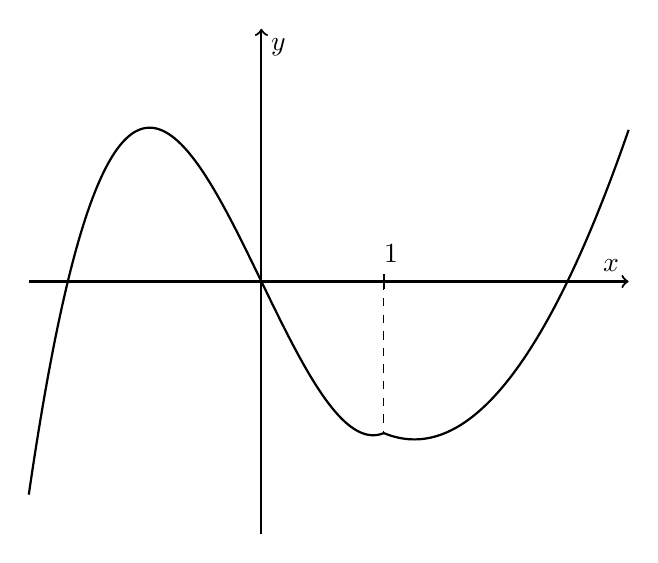
\begin{tikzpicture}
\begin{axis}[
    axis lines=middle,
    xmin=-1.9, xmax=3,
    ymin=-5, ymax=5,
    xlabel={$x$},
    ylabel={$y$},
    width=9.2cm,
    height=8cm,
    axis line style={->, thick},
    tick style={draw=none},
    xtick=\empty,
    ytick=\empty,
    clip=false,
    samples=150
]
\addplot[domain=-1.9:1, thick] {2*x^3-5*x};
\addplot[domain=1:3, thick] {2*x^2-5*x};
\addplot[dashed] coordinates {(1,0) (1,-3)};
\addplot[thick] coordinates {(1,-0.15) (1,0.15)};
\node at (axis cs:1.06,0.55) {$1$};

\end{axis}
\end{tikzpicture}
\end{center}

\bigskip
\hrule
\begin{center}
    This solution was submitted by \textbf{Camile}\\[4pt]
    Published and refined by \textbf{Jon}\\[8pt]
    \textit{Last updated: June 21, 2026}
\end{center}

\end{document}
